%
\documentclass[11pt]{article}
\usepackage[a4paper, margin=1in
]{geometry}
\usepackage{graphicx}
\usepackage{xcolor}
\usepackage{kpfonts}
\usepackage{fancyhdr}
\usepackage[
  style=ieee,
]{biblatex}
% use package for referencing figures
\usepackage{caption}
\usepackage{subcaption}
\usepackage[capitalise]{cleveref}

\usepackage[skip=1em]{parskip}

\pagestyle{fancy}

\title{\vspace{-2em}\small{Analysis of Week 12's Paper}\\\LARGE{Chromosal Organization through Loop Extrusion}\vspace{-1em}}
\author{Minghang Li}
\date{\vspace{-1em}}

\fancyhf{}
\lhead{Current Topics in Biophysics}
\rhead{\today}

\cfoot{\thepage}

\setlength{\parindent}{0ex}

\bibliography{report}

% -- end preamble --

\begin{document}

\maketitle \thispagestyle{fancy}

\bigskip
\hrule \vspace{1pt}
\hrule height 1pt
\bigskip

% the most important part it to explain

%  + what the general question is that is being addressed. that will include some general context on chromosome conformations and chromatin accessibility. (DONE!)
%  + how we learn about chromatin conformations (Hi-C etc) (DONE!)
%  * a discussion of the author's approach, the model, and the results.
%  * what the strength and weaknesses of the model are, what is left unexplained
%  * What could be done next? What has been done since?

% This discussion will include answers to many of the questions we discussed. You'll usually include some figures from the paper to make your point.

\begin{abstract}
  \noindent Week 12's lecture discussed the paper by Fudenberg et. al., titled by "\textit{Formation of Chromosomal Domains by Loop Extrusion}". It investigated the underlying mechanism of the formation of one of the most common and important chromosomal structure -- Topologically Associating Domains (TADs). It proposed the hypothesis that TADs are formed by loop extrusion regulated by Boundary Elements (BEs) and Loop Elongation Factors (LEFs) and tested the hypothesis through rigorous modelling and simulation.
\end{abstract}

\section{Background Introduction}

\subsection{Chromosomal Conformation Capture (3C) Technologies}

The genetic information stored in DNA sequences is not presented in a linear manner, but is rather folded and organized into three-dimensional (3D) structures, thereby allowing remotely located genomic elements interact with each other. To understand the 3D spatial genome organization better, various techniques have been developed over the years. Beyond the conventional microscopy observation that uncovered some basic principles about genome microscopy, the development of chromosome conformation capture (3C) technologies has also produced many important insights into the chromatin structure \cite{denker_second_2016}.

The 3C technology was first introduced in 2002 by Dekker et. al. originally in the hope of studying the folding of yeast chromosome \cite{dekker_capturing_2002}. It quickly inspired the emergence of an abundance of 3C-derived genomics methods. \cref{fig:3C} shows an overview of the 3C-derived technologies, which all start with the same steps. First, the DNA is crosslinked using a fixative agent, most often formaldehyde, to preserve the 3D representation of the genome. Second, the crosslinked DNA is digested with restriction enzymes to generate DNA fragments of a certain size. The DNA fragments are then ligated to specific adapters and amplified by PCR. The amplified DNA fragments are then sequenced and the sequence information is used to infer the spatial relationship between the captured DNA fragments \cite{wit_decade_2012}. Amongst all the 3C-derived technologies, Hi-C is probably the most widely used one. In Hi-C, the restriction ends of DNA fragments are filled in with biotin labeled nucleotides before the ligation step. Following a blunt ligation (usually by T4 DNA ligase), the biotin-labeled DNA fragments are purified and then captured by streptavidin-coated magnetic beads. After biotin-pulldown, the fragments are sheared into reads and then mapped back to the reference genome to generate a contact map, which is then used to score and infer the 3D structure of the genome \cite{wit_decade_2012}. Biotin pull-down and paired-end sequencing enables the detection of ligation junctions, and Next Generation Sequencing (NGS) methods makes such "all versus all" detection at a genome-wide scale possible.

% insert figure 1
\begin{figure}[htbp]
  \centering
  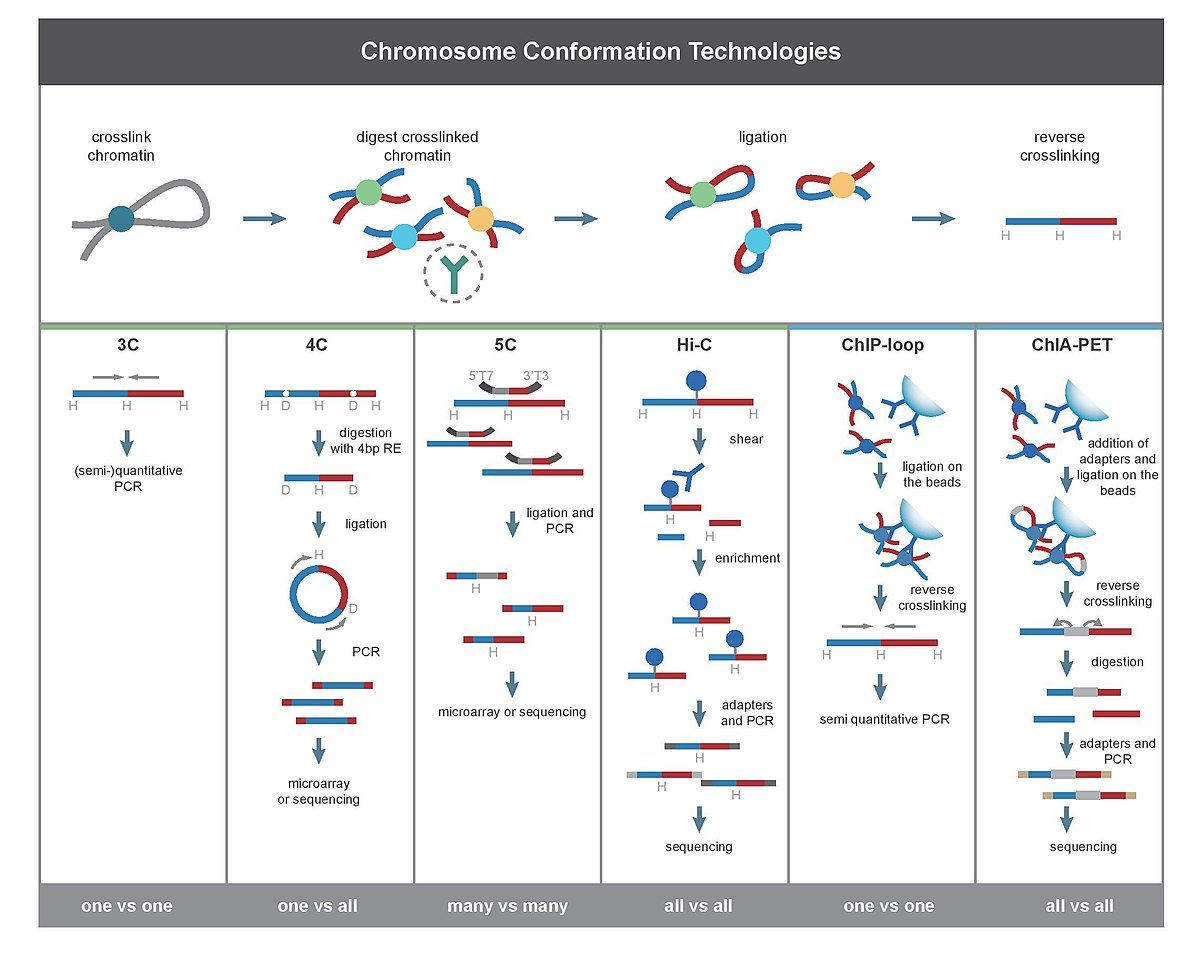
\includegraphics[width=0.8\textwidth]{assets/20221212064821.png}
  \caption{\textbf{An Overview of the 3C Technologies.}This figure comes from \cite{li_chromatin_2014}, which was adapted from \cite{wit_decade_2012}}
  \label{fig:3C}
\end{figure}

\subsection{Two Major Classes of Chromosomal Patterns}

Hi-C is capable of capturing the 3D structure of the genome at a resolution of kb level. In the Hi-C contact maps, two major classes of patterns are most evident. The first one is the A/B compartmentalization which shows checkerboard-like patterns \cite{mirny_two_2019}. The A compartment is usually gene-rich, transcriptionally active and accessible (characterized by DNase I sensitivity), and the B compartment is usually the heterochromatin region that is low in expression and has repressive histone marks \cite{denker_second_2016}\cite{wit_decade_2012}. The second one is the Topologically Associating Domains (TADs) which are characterized as continuous regions of mildly (2-4 folds) higher contact frequency than between loci in neighboring TADs \cite{mirny_two_2019}. They usually reside within a single contiguous compartment and don't necessarily exhibit the characteristic "checkerboard" pattern as A/B compartment does \cite{fudenberg_formation_2016}. 50\% of TADs have peaks of interactions at their boundaries, and they are capable of forming dynamic boundaries \cite{rao_3d_2014}. Up until the publishing of this paper, the formation of TADs was still not well understood. Previous works have proposed TADs forming mechanism based on similar monomer attraction \cite{jost_modeling_2014} and supercoiling \cite{benedetti_models_2014}, yet they fail to explain the formation of TADs in a satisfactory manner.

% \subsection{\textit{Cis}-Elements and \textit{Trans}-Factors Known to Involve in Maintaining Chromosomal Domains}

\subsection{CTCF, Cohesin, SMC}

To be finished.

% insert figure 2
\begin{figure}[htbp]
  \centering
  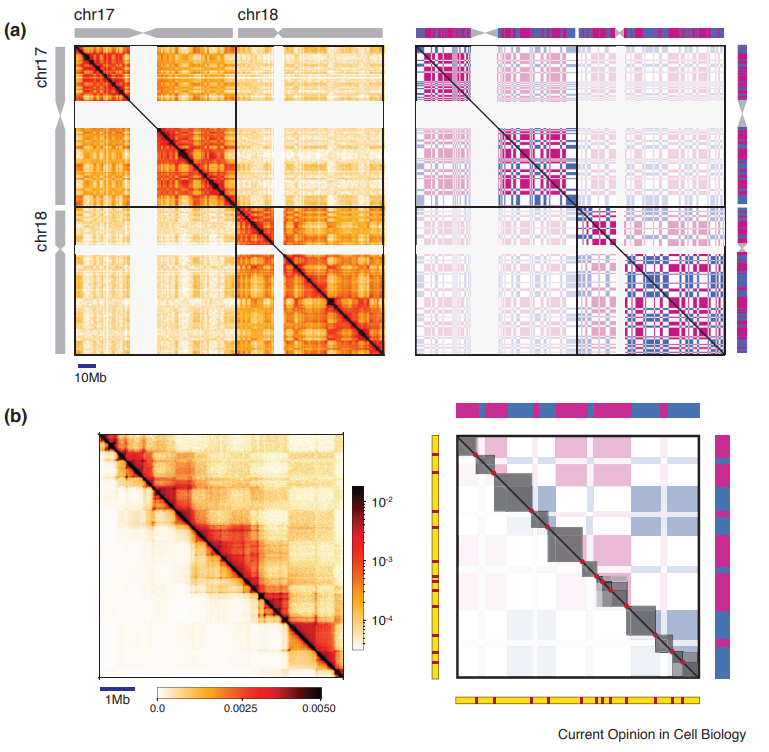
\includegraphics[width=0.8\textwidth]{assets/Snipaste_2023-01-13_15-53-18.png}
  \caption{\textbf{Hallmark Patterns in Hi-C Maps: Compartmentalization and TADs.} This figure comes from \cite{mirny_two_2019}. Fig (a) shows the A/B compartmentalization pattern, and Fig (b) shows the TADs pattern.}
  \label{fig:TAD}
\end{figure}

\section{Brief Summary of the Model}

To give out a satisfactory explanation for TAD formation, the authors proposed a loop-extrusion based mechanism. In this process, TADs are formed through the dynamic introduction of chromatin loop by \textit{cis}-acting loop-extruding factors (LEFs) and are bounded by boundary elements (BEs). The loop extrusion process was modelled by coupling the 1D dynamics of LEFs with 3D polymer dynamics. The following subsections will give a concise summary of the details of the proposed mechanism.

\subsection{Basic Settings of the 1-D Model}

The authors first defined the dynamics of LEFs with BEs. The translocation of LEFs along the chromatin fiber was simulated on a 1D lattice, where each position was characterized by association (birth) probability, dissociation (death) probability and BE occupancy (stalling probability). The LEF molecule was modelled by "two heads" connected with a linker, analogous to SMC protein complexes. Each head of the LEF occupied one lattice position and cannot be overlapped except for at birth events. At each time-step, each LEF head translocates to the neighboring lattics position in opposite direction until encountering another LEF head or a boundary element (BE). The stalling of one LEF head does not affect the translocation of the other LEF head.
At each discrete unit of time, a LEF undergoes dissociation with a probability that is equal to the maximum value of the death probability. For the occurrence of birth events, the two heads of the LEF are either initiated on the same lattice location or on neighboring sites (when the site immediately to the right of the selected site is unoccupied) with a probability of 0.5. The dynamics of LEFs were depicted in \cref{fig:LEF dynamics}.

% insert figure 3
\begin{figure}[htbp]
  \centering
  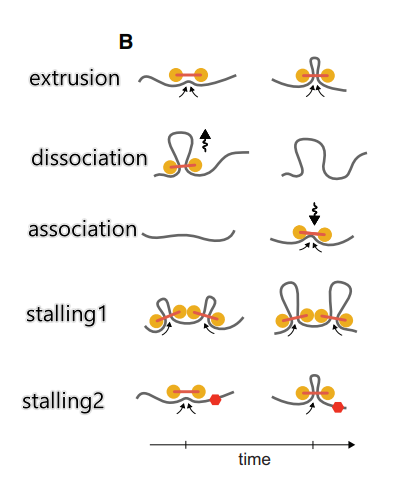
\includegraphics[width=0.5\textwidth]{assets/image-20221212095109951.png}
  \caption{\textbf{The Dynamics of LEFs.} This figure comes from \cite{fudenberg_formation_2016}.}
  \label{fig:LEF dynamics}
\end{figure}

\subsection{Basic Settings of the 3-D Polymer Model}

As is later shown in the paper, the 1-D model can very well depict the TAD as an average of experiments from many cells, yet it is difficult to model insulation solely by the 1-D model. For example, an enhancer and promoter separated by 100kb can still come in contact in the 3D space. To account for this, the authors proposed a 3D polymer model to simulate the 3D structure of the chromatin fiber.

The 3D chromatin model is a polymer connected by 10-nm monomers (roughly the size of 3 nucleosomes or 600bp) subject to Langevin dynamics, which according to my understanding models the stochastic behavior of molecules in solvent. The monomers are further modelled by excluded volume interactions, which prohibits monomer overlapping, and are linked with harmonic bonds that restrict their relative position but allow for rotation in certain degrees (stiffness) and chain passing (which represents the activity of topoisomerase and enables loop twisting and loop inside loops).

\subsection{Connecting the 1-D and 3-D Models}

LEFs serve as the connection points between 1-D and 3-D models: they affects the monomers of the 3-D model by introducing additional harmonic bond between the monomers held by the two heads of the LEFs. The bond is constantly reassigned to increasingly separated pairs of monomers as the LEF heads move along the chromosome. Furthermore, before starting the 3D simulation, the 1D LEF dynamics was first run for 4 million steps to achieve convergence of LEF initial positions. At each 1-D simulation time step, according to the hyperparameter \textit{3D-to-1D dynamics}, the corresponding 3D Langevin dynamics simulations were performed before starting the 1D-simulation time steps.

\subsection{Important Parameters of the Model As A Whole}

To simplify the simulation effort and to account for the still-unknown biological setup of exact LEF dynamics parameters, the authors chose to first use a simple setting with uniform birth probability, constant death probability, a fix number of LEFs and a discrete nubmer of impermeable BEs. The parameters have been relaxed in latter explorations such as the permeability of BEs, or even different types of BEs. Under such scenario, the LEF dynamics can be well described by only two metrics: the LEF processivity ($\frac{2}{\text{death rate}}$) and LEF separation ($\frac{\text{total number of lattice sites}}{\text{number of LEFs}}$). The processivity accounts for the average size of the loop extruded by an LEF if not stopped early; and the separation represents the distance between two pairs of LEFs on average.

In the simulations, the authors tested various combinations of processivity and separation and analyzed the effects of these parameters on the shape of the TADs.

\section{Brief Summary of the Results}

\subsection{Evaluation of the Model}

The authors used a measurement called $P(s)$ (a function of genomic distance $s$) to test the ability of the model to reproduce Hi-C contact map data. They plotted $s-P(s)$ curves for the model and the experimental data they obtained and confirmed that the shapes are similar. To measure the reproduction quantitatively, they also determined the \textit{goodness of fit} using the geometric standard deviation of the ratios of the experimental data nad simulated $P(s)$ curves. Using such measures, the authors identified the best parameter settings (processivity and separation) to reproduce the experimental data.

% insert figure 4
\begin{figure}[htbp]
  \centering
  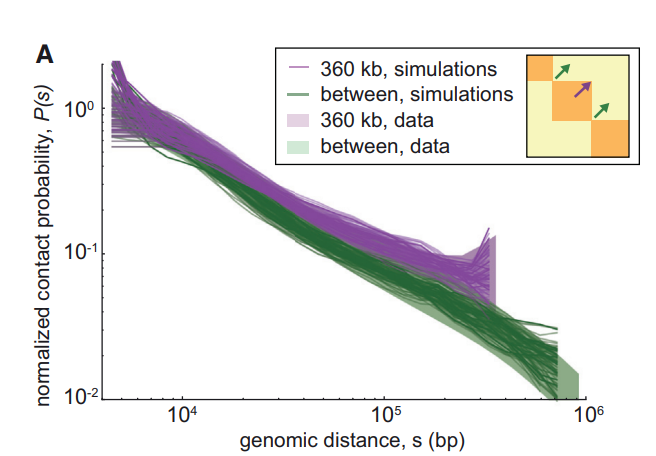
\includegraphics[width=0.8\textwidth]{assets/Snipaste_2023-01-13_17-49-12.png}
  \caption{\textbf{Evaluation of Model.} This figure comes from \cite{fudenberg_formation_2016}.  Experimental $P(s)$ (shaded areas) versus simulated $P(s)$ for the 100 best fitting parameter sets (lines, one per parameter set) within TADs (purple) and between
  TADs (green).}
  \label{fig:processivity and separation}
\end{figure}

\section{Strengths and Weaknesses of the Paper}

\section{Future Prospectives}

% Bibliography
\printbibliography

\end{document}
